\documentclass[12pt, letterpaper]{article}

% --- Packages ---
\usepackage{geometry}
 \geometry{margin=1in}
\usepackage{graphicx}
\usepackage{amsmath, amssymb}
\usepackage{booktabs}
\usepackage{hyperref}
\usepackage{cite}
\usepackage{setspace}
\onehalfspacing
\usepackage{fontspec}
\usepackage{polyglossia}
\usepackage{float}
\setmainlanguage{vietnamese}
\usepackage{listings}
\usepackage{xcolor}

% Define colors for syntax highlighting
\definecolor{mGreen}{rgb}{0,0.6,0}
\definecolor{mGray}{rgb}{0.5,0.5,0.5}
\definecolor{mPurple}{rgb}{0.58,0,0.82}
\definecolor{backgroundVisual}{rgb}{0.95,0.95,0.92}

\lstset{
    backgroundcolor=\color{backgroundVisual},
    commentstyle=\color{mGreen},
    keywordstyle=\color{magenta},
    numberstyle=\tiny\color{mGray},
    stringstyle=\color{mPurple},
    basicstyle=\footnotesize\ttfamily,
    breaklines=true,
    captionpos=b,
    keepspaces=true,
    numbers=left,
    numbersep=5pt,
    language=C,
    showstringspaces=false
}

% --- Metadata ---
\title{Báo cáo Lab2 - General purpose input/output programming}
\author{Đỗ Hoàng Gia Bảo - 23020783 \\ \small Khoa Điện tử - Viễn Thông \\ \small Giảng viên hướng dẫn: KS.Đỗ Đình Minh}
\date{\today}

\begin{document}

\maketitle

\begin{abstract}
Báo cáo sẽ trình bày các bước thực hiện các bài tập trong Lab2 và kết quả thu được của mỗi bài tập trên mạch NUCLEO-F401RE
\end{abstract}
% --- Front Matter (Roman Numerals) ---
\newpage
\tableofcontents

% --- Main Content (Arabic Numerals) ---
\newpage
\pagenumbering{arabic}
\setcounter{page}{3} % This automatically resets the counter to 1

\section{Exercise 1: Write a program to blink green LED on NUCLEO-F401RE board (using register)}
\subsection{Tìm PIN của vi điều khiển đảm nhiệm điều khiển LED xanh}
Trên bản thiết kế của mạch NUCLEO-F401RE, LED xanh được kết nối với chân PA5 của vi điều khiển NUCLEO-F401RE. Chân PA5 này có thể được sử dụng để điều khiển trạng thái của LED xanh bằng cách thiết lập hoặc xóa bit tương ứng trong thanh ghi GPIOA.
\begin{figure}[H]
    \centering
    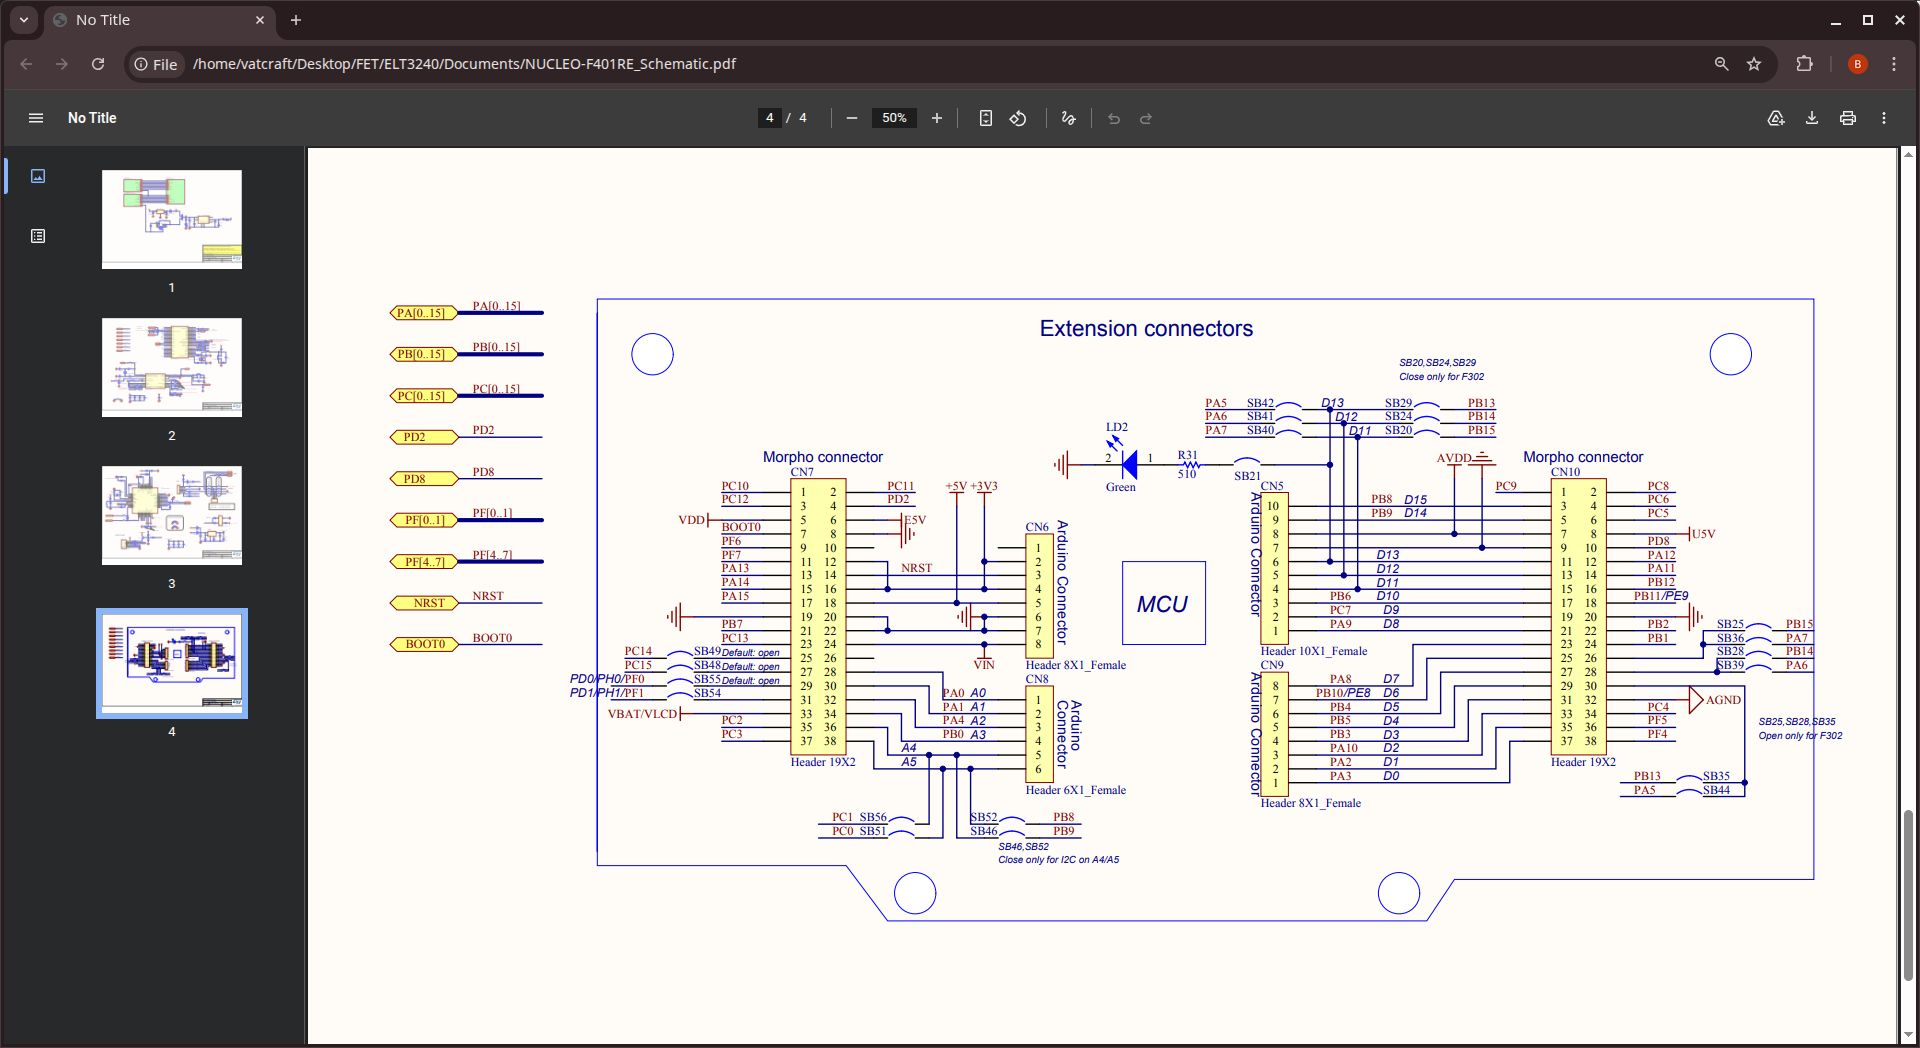
\includegraphics[width=0.8\textwidth]{schematic.jpg} 
    \caption{Sơ đồ kết nối của LED xanh với chân PA5 trên mạch NUCLEO-F401RE.}
    \label{fig:schematic}
\end{figure}
\subsection{Viết chương trình để nhấp nháy LED xanh}
Dưới đây là mã nguồn C điều khiển thanh ghi để nhấp nháy LED tại chân PA5:
\renewcommand{\lstlistingname}{Mã nguồn}
\lstinputlisting[language=C, caption=Chương trình điều khiển LED xanh qua thanh ghi]{../exercise1/exercise1/Core/Src/main.c}
Trong hàm main, chúng ta thực hiện các bước sau:
\begin{itemize}
    \item Kích hoạt clock cho GPIOA bằng cách thiết lập bit tương ứng trong thanh ghi RCC->AHB1ENR.
    \item Cấu hình chân PA5 là output bằng cách thiết lập bit tương ứng trong thanh ghi GPIOA->MODER.
    \item Sử dụng vòng lặp vô hạn để nhấp nháy LED bằng cách thiết lập và xóa bit tương ứng trong thanh ghi GPIOA->ODR thông qua thanh ghi GPIOA->BSRR.
\end{itemize}
\subsection{Kết quả}
Khi chạy chương trình trên mạch NUCLEO-F401RE, LED xanh sẽ nhấp nháy như trong video
\href{https://drive.google.com/file/d/1IqiOymMTAEUHK13-rBezX32JjWYP5Uq0/view?usp=sharing}{Video kết quả Exercise 1}.\\
Kết quả cho thấy LED xanh đã nhấp nháy đúng theo yêu cầu, chứng tỏ chương trình đã hoạt động chính xác.
\section{Exercise 2: Write a program to turn on green led on NUCLEO-F401RE board when pressing user
button and vice versa (using register)}
\subsection{Tìm PIN của vi điều khiển đảm nhiệm điều khiển nút nhấn}
Trên mạch NUCLEO-F401RE, nút nhấn người dùng (USER BUTTON) được kết nối với chân PC13 của vi điều khiển. Chân PC13 này có thể được sử dụng để đọc trạng thái của nút nhấn bằng cách kiểm tra bit tương ứng trong thanh ghi GPIOC->IDR.
\begin{figure}[H]
    \centering
    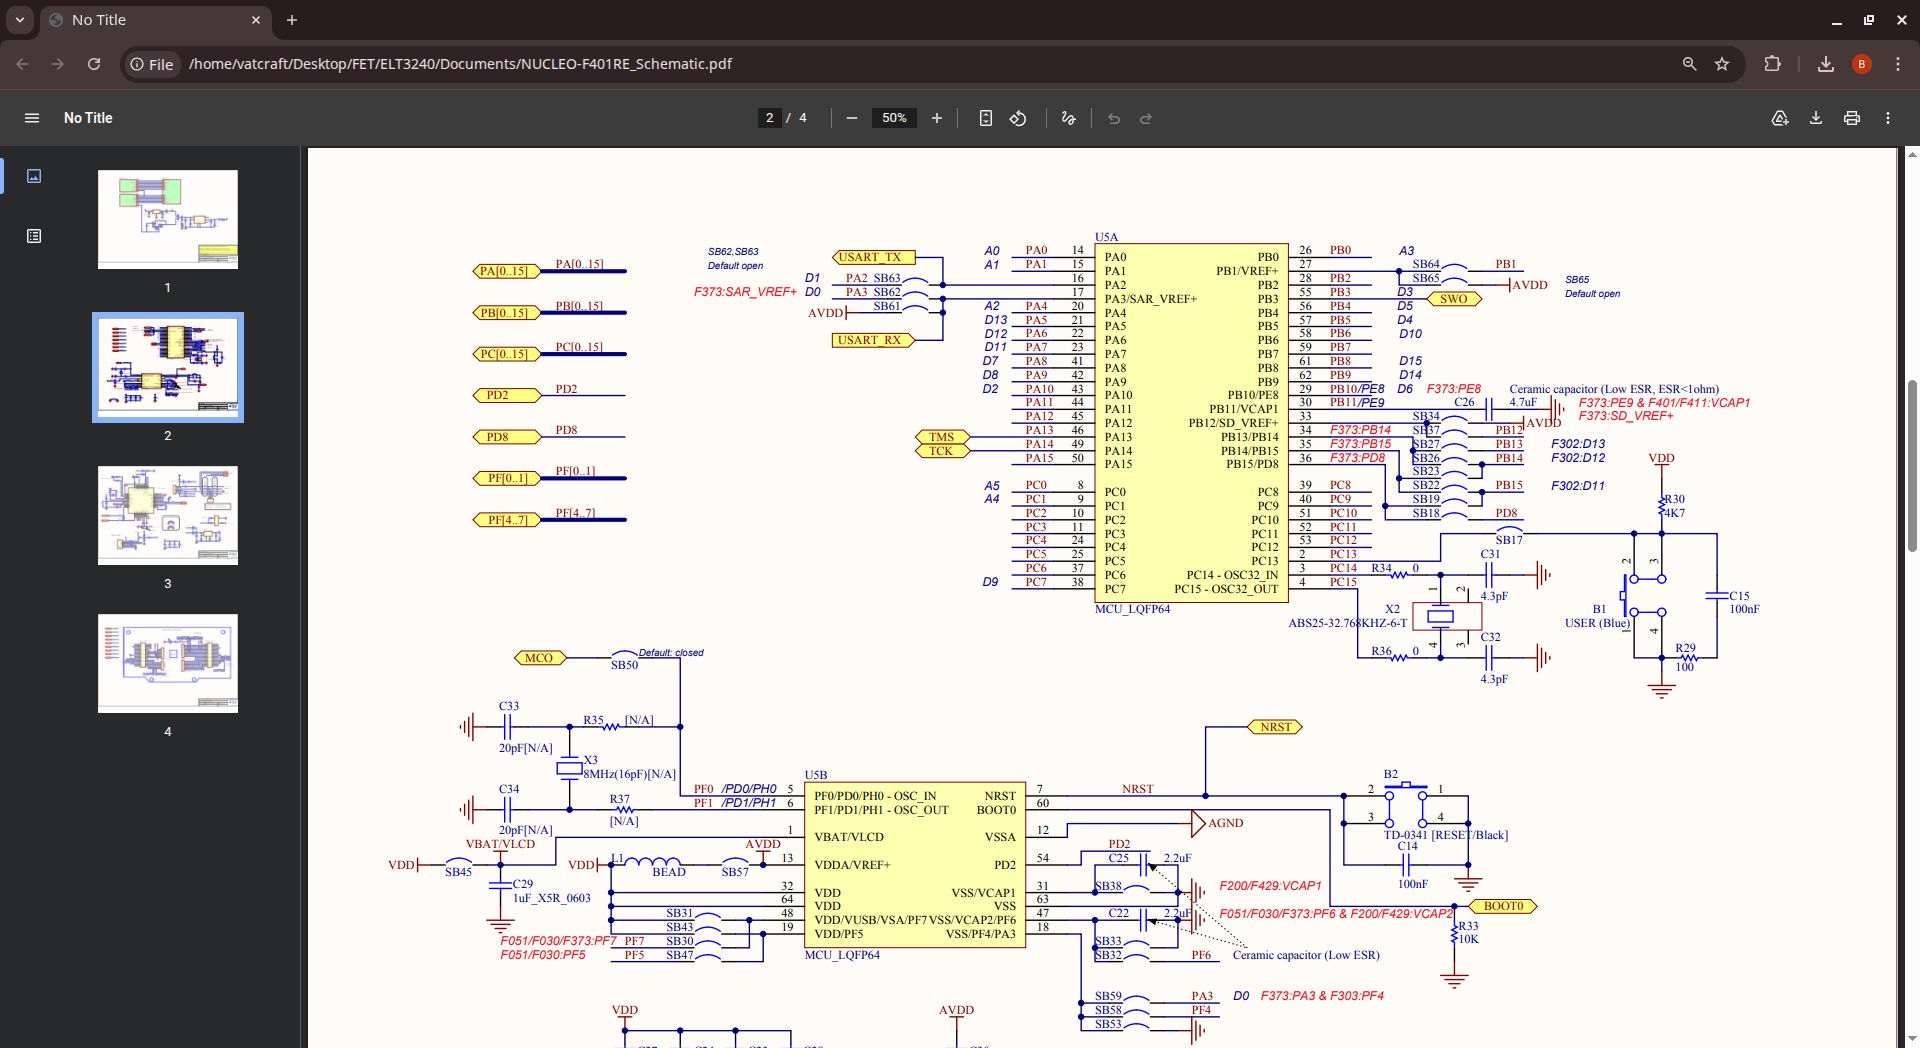
\includegraphics[width=0.8\textwidth]{schematic2.jpg} 
    \caption{Sơ đồ kết nối của nút nhấn người dùng với chân PC13 trên mạch NUCLEO-F401RE.}
    \label{fig:schematic2}
\end{figure}
\subsection{Viết chương trình để điều khiển LED xanh}
Dưới đây là mã nguồn C điều khiển thanh ghi để bật LED xanh khi nhấn nút và tắt khi thả nút:
\lstinputlisting[language=C, caption=Chương trình điều khiển LED xanh qua thanh ghi với nút nhấn]{../exercise2/Core/Src/main.c}
Trong hàm main, chúng ta thực hiện các bước sau:
\begin{itemize}
    \item Kích hoạt clock cho GPIOA và GPIOC bằng cách thiết lập bit tương ứng trong thanh ghi RCC->AHB1ENR.
    \item Cấu hình chân PA5 là output và chân PC13 là input bằng cách thiết lập bit tương ứng trong thanh ghi GPIOA->MODER và GPIOC->MODER.
    \item Sử dụng vòng lặp vô hạn để kiểm tra trạng thái của nút nhấn bằng cách đọc bit tương ứng trong thanh ghi GPIOC->IDR. Nếu nút nhấn được nhấn (bit tương ứng là 0), bật LED xanh bằng cách thiết lập bit tương ứng trong thanh ghi GPIOA->BSRR. Nếu nút nhấn được thả (bit tương ứng là 1), tắt LED xanh bằng cách thiết lập bit tương ứng trong thanh ghi GPIOA->BSRR.
\end{itemize}
\subsection{Kết quả}
Khi chạy chương trình trên mạch NUCLEO-F401RE, LED xanh sẽ bật khi nhấn nút và tắt khi thả nút như trong video
\href{https://drive.google.com/file/d/1M3ls7951JZR6aj7JM57I3B5hiynMz2xX/view?usp=sharing}{Video kết quả Exercise 2}.\\
Kết quả cho thấy LED xanh đã hoạt động đúng theo yêu cầu, chứng tỏ chương trình đã hoạt động chính xác.
\end{document}